\documentclass[a4paper]{report}

\usepackage[utf8]{inputenc}      % For setting up the encoding so you can type diacricts, e.g. é, ö.
\usepackage{geometry}            % For setting the correct papersize.
\usepackage[hidelinks]{hyperref} % Hyperlinks
\usepackage{graphicx}            % Images
\usepackage{rutitlepage}         % Titlepage

\begin{document}

\maketitleru[
	authors={Ruben Koelewijn \\s1105300},
	date={\today},
	others={%
		{First supervisor/assessor:}{Title(s) Firstname Lastname},
		{Second assessor:}{Title(s) Firstname Lastname}},
	course={Bachelor's Thesis Computing Science},
	title={Evaluating and Validating the Information Extraction of a Music Newsletter LLM},
	subtitle={Subtitle if you like},
	colour,
]

\begin{abstract}
% Brief outline of research questions, results.
% (The preferred size of an abstract is one paragraph or one page of text.)
Large language models (LLMs) are increasingly deployed in automated content pipelines, yet remain prone to hallucination, particularly when processing niche, localized information about entities underrepresented in their training data. This thesis addresses hallucination detection in one-sentence LLM-generated summaries of local music venue events, a domain where popularity bias renders both generative models and "LLM-as-a-judge" evaluation approaches unreliable.

We propose and evaluate a hybrid two-phase evaluation architecture that decouples reading comprehension from world knowledge verification. In the first phase, a cross-lingual Natural Language Inference model (XLM-RoBERTa) evaluates semantic entailment between English atomic claims, extracted via a deterministic spaCy dependency parser, and their Dutch source texts, detecting intrinsic hallucinations without an intermediate translation step. In the second phase, an external knowledge graph (MusicBrainz) provides deterministic, non-parametric overrides for extrinsic hallucinations that the NLI model alone cannot resolve.

Evaluated on 47 newsletter summaries from the Nijmegen venue Doornroosje, the baseline NLI pipeline achieved a sentence-level F1-score of 0.8615 and a perfect error detection rate of 1.0000, though at the cost of a high false positive rate of 0.4737. Knowledge graph integration successfully reclassified 5 atomic claims from extrinsic to intrinsic contradictions with 60\% accuracy, demonstrating particular strength in verifying geographic origin claims. However, due to strict min-pooling aggregation, these atomic corrections did not propagate to sentence-level improvements.

These findings demonstrate that a deterministic hybrid NLI and knowledge graph architecture is a methodologically sound alternative to circular LLM-based evaluation for niche, localized entity information, while identifying knowledge graph scope and aggregation strategy as the primary bottlenecks for future improvement.

The full Github Repository can be found at \url{https://github.com/rkoelewijn/bachelor-thesis}
\end{abstract}


\tableofcontents

\chapter{Introduction}\label{introduction}
% \textcolor{red}{The introduction of your bachelor thesis introduces the research area, the research hypothesis, and the scientific contributions of your work.
% A good narrative structure is the one suggested by Simon Peyton Jones~\cite{peys04:HowToWriteAGoodResearchPaper}:}

% \begin{itemize}
% 	\item \textcolor{red}{describe the problem \slash{} research question}
% 	\item \textcolor{red}{motivate why this problem must be solved}
% 	\item \textcolor{red}{demonstrate that a (new) solution is needed}
% 	\item \textcolor{red}{explain the intuition behind your solution}
% 	\item \textcolor{red}{motivate why \slash{} how your solution solves the problem (this is technical)}
% 	\item \textcolor{red}{explain how it compares with related work}
% \end{itemize}

% \textcolor{red}{Close the introduction with a paragraph in which the content of the next chapters is briefly mentioned (one sentence per chapter).}



% - TALK ABOUT RISE OF LLM USAGE SINCE 2020 - introduction of problem
In recent years, large language models (LLMs) have emerged and evolved rapidly \cite{zhao2023survey}. While initially restricted to research environments, these tools have now reached massive public scale. For instance, OpenAI recently confirmed it has surpassed 50 million paying subscribers across its commercial tiers, with up to 900 million weekly active users processing over 2 billion prompts per day \cite{openai2025enterprise}. This scale demonstrates that interacting with LLMs has become a routine global practice. However, while these models assist users in learning, working, and automating tasks, their widespread deployment does not come without downsides.

One primary risk is \textit{hallucination}, a phenomenon further discussed in Chapter \ref{preliminaries}, where an LLM generates output that is unfaithful to its original source or the user's instructions. While minor discrepancies often go unnoticed, severe hallucinations can have profound consequences. For example, Zhao \etal \cite{zhoa2026llmhallucinationsinthewild} analyzed 2.5 million published papers and found a sharp rise in non-existent references following widespread LLM adoption, conservatively estimating over 146,000 hallucinated citations in 2025 alone. Similar impacts have been documented across other critical sectors. In healthcare, hallucinations pose severe ethical and safety risks \cite{healthcarehallucinations2025}, while in the commercial sector, the use of ungrounded conversational agents has led to concrete operational liabilities for enterprises \cite{lseo2026liability}.

As mentioned above, the occurrences of hallucinations are well-documented in high-stakes fields like medicine and law. 
In this thesis, however, we will consider a use-case which is less universally known, a case on a local music venue in Nijmegen. 
Since local venues often give the stage to smaller, lesser-known artists, the likelihood of hallucinations increases. While large language models demonstrate impressive factual recall for globally prominent topics, their reliability degrades significantly when processing niche or localized information. This limitation, often referred to as popularity bias, is formally quantified by Kandpal \etal \cite{kandpal2023longtail}, who demonstrate that an LLM's ability to accurately state a fact is directly correlated to the frequency of that entity's appearance in its pre-training corpus.

To address these widespread hallucinations, a common modern approach is the ``LLM-as-a-judge'' solution, wherein a highly capable model (such as GPT-4) is prompted to verify the factual accuracy of generated text. However, recent benchmarking reveals critical structural flaws in this methodology. Chen \etal \cite{chen2023felm} introduced the FELM benchmark, demonstrating that LLM evaluators struggle significantly to detect factual errors, often failing to identify hallucinations or confidently hallucinating false corrections themselves. This failure occurs because an LLM acting as a judge relies on the same flawed, popularity-biased parametric memory as the model generating the text, where a parametric memory refers to a models internal knowledge determined by the models internal knowledge. If an LLM lacks the training data to accurately describe a local Dutch punk band, it also lacks the data required to fact-check a summary about that band. Consequently, relying on an LLM to evaluate long-tail cultural metadata creates a circular validation flaw.

To solve this, a new approach to automated evaluation is required. Traditional hallucination benchmarks often evaluate models against static, global datasets and primarily focus purely on English tasks. 
These traditional measures where not set up with testing small scale musical knowledge in mind, where the source text differs from the summarisation. 

Therefore, we propose a two-phase hybrid evaluation architecture designed specifically for this domain.

The intuition behind this solution is to split the evaluation into two distinct steps: confirming the source text was understood, and checking if the claims match reality. First, to assess whether the LLM faithfully translated and summarized the provided text, we utilize a cross-lingual Natural Language Inference (NLI) model (XLM-RoBERTa). This isolates intrinsic hallucinations. Second, to overcome the LLM's popularity bias regarding long-tail entities, we integrate a non-parametric, structured external database (MusicBrainz). By deterministically cross-referencing the LLM's claims against this real-world knowledge graph, we can catch extrinsic hallucinations that the NLI model alone would miss. Using manually labelled claims, we compare the accuracy of our built pipeline and are able to identify wide range of hallucinations types. 


Our primary research question entails: 
\begin{enumerate}
    \item[\textbf{RQ 1}] To what extent can a hybrid evaluation framework, integrating deterministic claim decomposition, cross-lingual Natural Language Inference (NLI), and a structured external knowledge graph, effectively detect and categorize hallucinations in one-sentence LLM-generated local music venue summaries?
    \begin{enumerate}
        \item[\textbf{RQ 1.1}] How accurately can the cross-lingual NLI baseline pipeline detect and classify intrinsic hallucinations by evaluating semantic entailment between English atomic claims and their Dutch source texts, and to what extent does it label extrinsic hallucinations with a neutral or supported verdict?
        \item[\textbf{RQ 1.2}] How does the calibration of the baseline confidence threshold ($\mathcal{T}$) impact the models error detection and accuracy? 
        \item[\textbf{RQ 1.3}] How effectively can the integration of the MusicBrainz external knowledge graph increase the accuracy of atomic and sentence level labels of the baseline by validating extrinsic and intrinsic hallucinations?
        \item[\textbf{RQ 1.4}] How does aggregating these atomic claim-level evaluations using min-pooling impact the  error detection and false positive rates at the sentence level?
    \end{enumerate}
\end{enumerate}

The remainder of this thesis is structured as follows. Chapter \ref{preliminaries} outlines the theoretical background regarding hallucinations in LLMs, cross-lingual NLI, Knowledge Graphs and Binary Classification Metrics. Next, Chapter \ref{Newsletter} discusses the used dataset, how it was generated and what existing problems occur. Following this, Chapter \ref{research} discusses the full evaluation pipeline architecture, including generating the corpus, extracting source data and the external knowledge graph, parsing Dutch source text, decomposing the summaries into atomic claims, validating and evaluating these atomic claims and lastly the experiment set up. Chapter \ref{results} shows the results of our experiments, which will then be discussed in Chapter \ref{discussion} and future work will be suggested in addition to our limitations . Finally, Chapter \ref{conclusions} concludes the research by answering the research questions according to our results and discussion.





\chapter{Preliminaries}\label{preliminaries}
This \emph{optional} chapter contains the stuff that your reader needs to know in order to understand
your work.
Your ``audience'' consists of fellow third year computing science bachelor students who have done the same
core courses as you have, but not necessarily the same specialization, minor, or free electives.

You do not have to call this chapter \emph{Preliminaries} and it does not need to be limited to one chapter.
Some preliminary topics deserve their own chapter.

\textbf{Preliminaries:}
\begin{itemize}
    \item LLM Hallucination
    \item Cross-Lingual Natural Language Inference (NLI)
    \item Open Web Index (OWI) Architecture \todo[color=gray,nolist]{If i decide on using it.}
\end{itemize}


\section{Hallucination in Large Language Models}\label{pre:sec:llm}
In this thesis, we will be looking at the output of different Large Language Models (LLM). LLMs are massive artificial neural networks
pre-trained on vast amounts of text data, designed to understand and generate human language. They show strong understanding in natural language and solving 
complex tasks.  \cite{zhao2023survey} While these outputs often contain useful and correct information, they are prone to \textit{hallucinating}. 
Hallucination of a LLM consists of the model generating content that is not faithful to its source. There exist multiple types of hallucinating, 
and following the taxonomy proposed by
\cite{huang2025survey}, we can categorise these into two types: 
\begin{itemize}
    \item \textbf{Factuality Hallucinations} 
    \\ Discrepancies between generated content and verifiable real-world facts. 
    This includes \textit{Fabrications} (made-up claims) and \textit{Contradictions} (statements that directly oppose reality).
    \item \textbf{Faithfulness Hallucinations} 
    \\ Divergence from the provided user input or context. This includes \textit{Instruction} (following the wrong instructions from the prompt), 
    \textit{Context} (Not understanding the context) and \textit{Logical} (Incorrect logic, e.g. math errors).  
    In information extraction (IE) tasks, these often manifest as ``Missing Spans" or ``Incorrect Types" \cite{gao2024empirical}.
\end{itemize}

\noindent Classifying the LLM Hallucination, allows us to have insight on what went wrong and where to improve. It gives us the ability to do a system-level
diagnosis of the pipline \cite{vinay2025failuremodesllmsystems}. For instance, a \textit{faithfulness} error indicates a failure to maintain ``context-boundary" stability \cite{vinay2025failuremodesllmsystems}, 
where a \textit{factuality} error might need external grounding through retrieval. Because LLMs are often unable to faithfully detect their own factual errors 
  \cite{chen2023felm}, deterministic verification is required to ensure airtight verification. 



\section{Cross-Lingual Natural Language Inference}\label{pre:sec:nli}
Natural Language Inference (NLI), also known as Recognizing Textual Entailment (RTE), 
is a core task in Natural Language Processing (NLP) \cite{conneau2020unsupervised}. 
NLP is a multidisciplinary field at the crossover between Computing Science, Linguistics, and Artificial Intelligence, where scientists focus on 
helping computers understand natural language. Common applications consist of machine translation, 
sentiment analysis, and automated summarisation. The latter is 
highly relevant for this thesis, since we deal with Information Extraction (IE), specifically
 extracting text and entities from websites \cite{gao2024empirical}, and Semantic Validation, 
 which involves logically validating the semantic meaning of different sentences to detect errors \cite{huang2025survey, chen2023felm}.

The task of NLI in NLP is determining the logical relationship between two pieces of text: 
a \textit{premise} and a \textit{hypothesis} \cite{conneau2020unsupervised}. Based on the truth of the premise, 
the model assigns one of three categorical labels as demonstrated in Table \ref{tab:nli_examples}:

\begin{table}[h]
    \centering
    \caption{Examples of Natural Language Inference (NLI) relationships.}
    \label{tab:nli_examples}
    \begin{tabular}{lll}
        \toprule
        \textbf{Premise} & \textbf{Hypothesis} & \textbf{NLI Label} \\
        \midrule
        Frank Boeijen is from Nijmegen. & Nijmegen is the hometown of Frank Boeijen. & \textit{Entailment} \\
        Frank Boeijen is from Nijmegen. & Frank Boeijen is from Amsterdam. & \textit{Contradiction} \\
        Frank Boeijen is from Nijmegen. & Frank Boeijen is coming back to Nijmegen. & \textit{Neutral} \\
        \bottomrule
    \end{tabular}
\end{table}

\begin{itemize}
    \item \textbf{Entailment:} The hypothesis is guaranteed to be true if the premise is true. In Table \ref{tab:nli_examples}, 
    the premise logically necessitates that Nijmegen is Boeijen's hometown \cite{conneau2020unsupervised}.
    \item \textbf{Contradiction:} The hypothesis is guaranteed to be false if the premise is true. 
    Since the premise establishes Nijmegen as the origin, a claim of Amsterdam constitutes a direct contradiction \cite{conneau2020unsupervised}.
    \item \textbf{Neutral:} The truth of the hypothesis cannot be determined from the premise alone. 
    While Frank Boeijen may be ``coming back" to Nijmegen, the original premise regarding his origin does not provide sufficient
     information to confirm or deny a return trip \cite{conneau2020unsupervised}.
\end{itemize}

\noindent In the context of this thesis, we utilize \textit{Cross-Lingual} NLI to bridge the language gap 
between Dutch source text and English generated summaries. By using a multilingual model like XLM-RoBERTa, 
we can evaluate a Dutch premise against an English hypothesis without an intermediate translation step,
 preserving the semantic nuances of the original concert metadata \cite{conneau2020unsupervised}.
\chapter{Research}\label{research} \todo{Change Title}
This chapter, or series of chapters, delves into all technical details that are required to \emph{prove} your scientific hypothesis.
Please do not call this chapter or these chapters \emph{Research} as that name is not descriptive.
It should be sufficiently detailed and precise in order for any fellow computing scientist student to be able to \emph{repeat} your research and therewith establish the same results \slash{} conclusions that you have obtained.
Please note that, in order to improve readability of your thesis, you can put a part of this information also in one or more appendices (see Appendix~\ref{appendix}).


\section{Pipeline Setup}
In order to correctly verify the summary given by the LLM model, we have to create a pipeline that sources the needed context. As seen in Chapter \ref{Newsletter}, the newsletter contains a one-sentence summary. Before we can validatie whether this is true or not, we need to extract all context. This is done by loading the URL using a headless browser, where we scrape the Dutch text. This then gets parsed and cleaned, and sent to the validator. Meanwhile, the summary gets chopped into atomic claims, who then can be validated. A diagram can be found in figure \ref{fig:pipeline_flowchart}. 
\begin{figure}[htbp]
\centering
\tikzset{every picture/.style={line width=0.75pt}} %set default line width to 0.75pt        

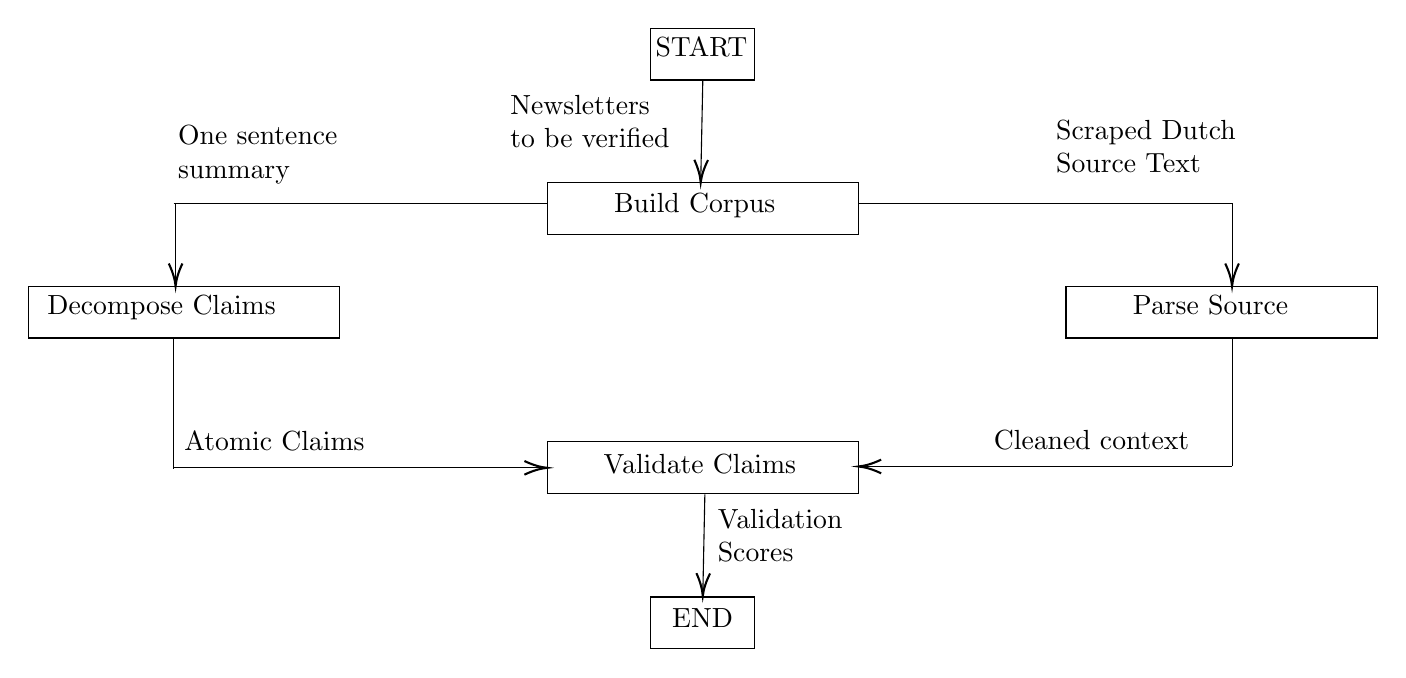
\begin{tikzpicture}[x=0.75pt,y=0.75pt,yscale=-1,xscale=1]
%uncomment if require: \path (0,680); %set diagram left start at 0, and has height of 680

%Shape: Rectangle [id:dp4070963882781028] 
\draw   (300,1) -- (350,1) -- (350,25.96) -- (300,25.96) -- cycle ;
%Shape: Rectangle [id:dp9774405992082825] 
\draw   (250,75.38) -- (400,75.38) -- (400,100.33) -- (250,100.33) -- cycle ;
%Straight Lines [id:da38434376573046714] 
\draw    (325,26.46) -- (324.04,73.38) ;
\draw [shift={(324,75.38)}, rotate = 271.17] [color={rgb, 255:red, 0; green, 0; blue, 0 }  ][line width=0.75]    (10.93,-3.29) .. controls (6.95,-1.4) and (3.31,-0.3) .. (0,0) .. controls (3.31,0.3) and (6.95,1.4) .. (10.93,3.29)   ;
%Shape: Rectangle [id:dp7238715529174791] 
\draw   (0,125.29) -- (150,125.29) -- (150,150.25) -- (0,150.25) -- cycle ;
%Shape: Rectangle [id:dp544713314300144] 
\draw   (500,125.29) -- (650,125.29) -- (650,150.25) -- (500,150.25) -- cycle ;
%Shape: Rectangle [id:dp6187874396247628] 
\draw   (250,200.17) -- (400,200.17) -- (400,225.13) -- (250,225.13) -- cycle ;
%Shape: Rectangle [id:dp9525801403683838] 
\draw   (300,275.04) -- (350,275.04) -- (350,300) -- (300,300) -- cycle ;
%Straight Lines [id:da7731746387458769] 
\draw    (580,85.36) -- (580,123.29) ;
\draw [shift={(580,125.29)}, rotate = 270] [color={rgb, 255:red, 0; green, 0; blue, 0 }  ][line width=0.75]    (10.93,-3.29) .. controls (6.95,-1.4) and (3.31,-0.3) .. (0,0) .. controls (3.31,0.3) and (6.95,1.4) .. (10.93,3.29)   ;
%Straight Lines [id:da8488203549026855] 
\draw    (400,85.36) -- (580,85.36) ;

%Straight Lines [id:da17279727340281192] 
\draw    (580,212.15) -- (402,212.15) ;
\draw [shift={(400,212.15)}, rotate = 360] [color={rgb, 255:red, 0; green, 0; blue, 0 }  ][line width=0.75]    (10.93,-3.29) .. controls (6.95,-1.4) and (3.31,-0.3) .. (0,0) .. controls (3.31,0.3) and (6.95,1.4) .. (10.93,3.29)   ;
%Straight Lines [id:da7845149368668756] 
\draw    (580,150.25) -- (580,212.15) ;

%Straight Lines [id:da8313227318576999] 
\draw    (326,225.62) -- (325.04,272.54) ;
\draw [shift={(325,274.54)}, rotate = 271.17] [color={rgb, 255:red, 0; green, 0; blue, 0 }  ][line width=0.75]    (10.93,-3.29) .. controls (6.95,-1.4) and (3.31,-0.3) .. (0,0) .. controls (3.31,0.3) and (6.95,1.4) .. (10.93,3.29)   ;
%Straight Lines [id:da5767226057733228] 
\draw    (71,85.36) -- (71,123.29) ;
\draw [shift={(71,125.29)}, rotate = 270] [color={rgb, 255:red, 0; green, 0; blue, 0 }  ][line width=0.75]    (10.93,-3.29) .. controls (6.95,-1.4) and (3.31,-0.3) .. (0,0) .. controls (3.31,0.3) and (6.95,1.4) .. (10.93,3.29)   ;
%Straight Lines [id:da09197572758197181] 
\draw    (70,85.36) -- (250,85.36) ;

%Straight Lines [id:da9262340614866109] 
\draw    (70,212.8) -- (248,212.8) ;
\draw [shift={(250,212.8)}, rotate = 180] [color={rgb, 255:red, 0; green, 0; blue, 0 }  ][line width=0.75]    (10.93,-3.29) .. controls (6.95,-1.4) and (3.31,-0.3) .. (0,0) .. controls (3.31,0.3) and (6.95,1.4) .. (10.93,3.29)   ;
%Straight Lines [id:da6502941044352438] 
\draw    (70,213.15) -- (70,150.25) ;


% Text Node
\draw (281,79.11) node [anchor=north west][inner sep=0.75pt]   [align=left] {Build Corpus};
% Text Node
\draw (531,128.52) node [anchor=north west][inner sep=0.75pt]   [align=left] {Parse Source};
% Text Node
\draw (276,204.89) node [anchor=north west][inner sep=0.75pt]   [align=left] {Validate Claims};
% Text Node
\draw (231,31.92) node [anchor=north west][inner sep=0.75pt]   [align=left] {Newsletters \\to be verified};
% Text Node
\draw (494,43.88) node [anchor=north west][inner sep=0.75pt]   [align=left] {Scraped Dutch \\Source Text};
% Text Node
\draw (464,193.41) node [anchor=north west][inner sep=0.75pt]   [align=left] {Cleaned context};
% Text Node
\draw (71,46.87) node [anchor=north west][inner sep=0.75pt]   [align=left] {One sentence \\summary};
% Text Node
\draw (74,193.91) node [anchor=north west][inner sep=0.75pt]   [align=left] {Atomic Claims};
% Text Node
\draw (8,128.52) node [anchor=north west][inner sep=0.75pt]   [align=left] {Decompose Claims};
% Text Node
\draw (331,231.58) node [anchor=north west][inner sep=0.75pt]   [align=left] {Validation \\Scores};
% Text Node
\draw (309,279.27) node [anchor=north west][inner sep=0.75pt]   [align=left] {END};
% Text Node
\draw (301,4.23) node [anchor=north west][inner sep=0.75pt]   [align=left] {START};


\end{tikzpicture}
\caption{System architecture flowchart demonstrating the corpus ingestion, atomic claim decomposition branches, and cross-lingual source verification steps.}
\label{fig:pipeline_flowchart}
\end{figure}
Each paragraph will explain in depth the architectural choices that were made and how each part of the pipeline works. 

\subsection{Dataset and Corpus Construction} \label{rsh:datacorpus}
Before any validation or evaluation is possible, we need to load the source data given in the newsletters url part. This allows us to create a so-called \textit{corpus} which contains all available data we have on the artist we are evaluating.
This corpus is setup as a deterministic and sandboxed evaluation dataset, rather than executing live web scraping and external API queries during the NLI and KG evaluation phases. By doing all the data loading up front, we save time loading all data again when our pipeline crashes later on, or if we wish to run the experiment again. 

This process collects the data in three simple steps: loading the local venue data, fetching the MusicBrainz facts, and saving everything to a JSON file.

\subsubsection{Extracting Venue Data}
As mentioned in Chapter \ref{Newsletter}, our primary data source is a generated newsletter, where we will be focussing on the venue Doornroosje, located in Nijmegen. This is setup using an automated web scraper, where the primary event details and the LLM-generated summaries are manually extracted from these newsletters and provided to the script. 

A comprehensive breakdown of the newsletter generation process, including its structural and visual layout, is discussed later in Chapter \ref{ch:cloudspeakers_pipeline} (The Cloudspeakers Pipeline). For the purpose of constructing this evaluation corpus, the script strictly isolates the English promotional text—which serves as our target for hallucination detection—alongside the core billing metadata required to identify the performing artists.

\subsubsection{Gathering MusicBrainz Knowledge}
Once the primary event data is manually set up, the script automatically fills the dataset with verified real-world facts by querying the MusicBrainz API. To respect the strict rate-limiting policies enforced by the MusicBrainz infrastructure, the script utilizes a mandatory one-second delay between consecutive requests, ensuring the outbound traffic remains at or below $1 request \slash second$. 

For every artist identified in the venue data, the script searches the API to retrieve three specific data points: their geographic origin, associated musical genres, and any registered aliases. This factual data is stored to serve as the ground truth for detecting extrinsic hallucinations later in the pipeline. 

Given that mid-tier venues frequently program niche, emerging, or highly localized artists, it is expected that some acts will be entirely absent from the MusicBrainz database. To ensure the robustness of the dataset generation, the script implements explicit error handling. If an artist cannot be resolved, the pipeline catches the exception and assigns empty values to the factual fields rather than terminating the program, allowing the script to safely proceed to the next entity.


\subsection{Decomposer}\label{rsh:decomposer}
The main task of the decomposer step is to view the claims made by the LLM in the generated summary. A summary can contain from one untill multiple claims, so it is important that all of them get separated into atomic claims and get evaluated. We define a claim as `atomic' if it contains exactly one predicate-argument relationship, which allows the subsequent NLI model to render a definitive Entailment or Contradiction label without semantic noise.

While state-of-the-art frameworks like Google DeepMind's SAFE \cite{safe2024longform} rely on LLM prompting to decompose long-form summaries into atomic claim, introducing yet another machine learning model and creating high operational and computational costs, we made the choice to do this in a deterministic fashion. Our methodology adopts the core multi-stage atomic decomposition paradigm pioneered by SAFE, but replaces the LLM parser with a deterministic, rule-based linguistic dependency parse utilizing \texttt{spaCy}. Splitting claims into atomic claims, has been proven to improve performance in NLI for multiple models \cite{huang2026atomicsnlifinegrainednaturallanguage} and our own small scale testing (See Table \ref) \additions{Add table to show atomic claims give better results (maybe?)}. Our decomposer has been developed in parallel to the framework given by Huang et al. 


Crucially, by utilizing a deterministic linguistic dependency parser rather than a secondary LLM for claim decomposition, we avoid the `recursive hallucination' risk. When an LLM is used to decompose a summary, it may introduce its own hallucinations during the parsing phase. Our rule-based approach ensures that the decomposition remains faithful to the text's syntactic structure, effectively providing a stable, verifiable input for the subsequent NLI evaluation.

The core of our decomposer consists of treating a sentence as a hierarchical Dependency Tree, where words are nodes connected by functional relationships. These relationships mimic the function of words in English sentences, such as a \textit{preposition}, \textit{subject}, \textit{object}. The enumeration below shows the implementation of the algorithm. 
\begin{enumerate}
    \item Convert the raw text into a machine-readable dependency tree. This allows the system to identify the grammatical roles of words, such as which terms function as the subject and which function as the object of an action.
    \item Iterate through every token in the document to locate ``action anchors." The system prioritizes VERB and AUX (auxiliary verbs such as `is' or `has'), as these words define the core events or states necessary for a factual claim.
    \item Resolving Components: 
    \begin{itemize}
        \item Subject: Identify the nominal subject (`nsubj'). If the subject is a pronoun (e.g., ``He"), replace it with the primary entity name to ensure the claim remains contextually independent and verifiable.
        \item Verb Phrase: Collect all auxiliary verbs to preserve the original tense (e.g., ``is performing").
        \item Object: Locate the grammatical receiver of the action (direct object, attribute, or complement).
        \item Modifiers: Identify surrounding phrases that provide extra context, such as time, location, or manner.
    \end{itemize}
    \item  Combine the subject, verb phrase, and object to construct a coherent, standalone sentence that represents the core fact.
    \item If the sentence includes modifiers, ``multiply" the base statement by each modifier to generate individual, independent claims. This step converts one complex sentence into multiple simple, verifiable statements.
    \item  Perform final data hygiene. Remove exact duplicate claims and discard any fragments that are under 5 words in length. This ensures the final output contains only high-quality, meaningful information.
\end{enumerate}

\subsection{Dutch Parser}

\subsection{Validator}
\subsubsection{Theory}
Validating the claims is the core part of the operation we are doing. The validation is a process of cross-language NLI, comparing the original Dutch text to the English summaries that are given. 

% explain why we used RoBERTa over other choices 
To avoid the inherent bias of self-validation—where an LLM acts as an uncritical judge of its own generated output
\footnote{In the Netherlands, this specific conflict of interest is known as acting such as the company `WC-Eend', referencing
 a famous advertising campaign in which the brand recommends its own product (Wij van Wc-Eend adviseren Wc-Eend).}, \changes{move footnote to introduction.}
the option of using a generative model for the entailment check was discarded.
\textcolor{red}{Even though multiple studies have shown this to be effective, 
we wish to find a way to do this in a deterministic way due to LLMs having the nature of being unpredictable and prone to hallucination, 
as mentioned in section \ref{pre:sec:llm}. } 
\source{find the studies that show LLM can verify themselves.}
Comparing the premise and the hypothesis can be done in multiple ways, but for this thesis we have made the choice to make use of Facebook's XLM-RoBERTa \cite{conneau2020unsupervised}. 

XLM-RoBERTa, is a Transformer-based language model trained on 2.5 Terabytes of filtered CommonCrawl data across 100 different languages.
XLM-R learns a shared mathematical representation of human language, which results in it being able to convert multiple languages into a mapped mathematical vector space, meaning different languages can be compared. 
Conneau et al. show that XLM-R is very competitive with strong monolingual models on XNLI benchmarks, demonstrating that it is possible to have a single large model for all languages. \cite{conneau2020unsupervised} For the Cloudspeakers Experiment (section \ref{Newsletter}), this saves us steps from translating between Dutch and English, or limiting the experiments to pages that \textit{do} have an English variant. 
As mentioned in \ref{pre:sec:nli}, NLI looks at the entailment, contradiction and neutral scores. XLM-R outputs these when given a premise and hypothesis and using these we can determine likelihood of a hallucination by the LLM. 

Guidelines to the entailment scores can be found in Table XX. \additions{add table with entailment Guidelines}

\begin{verbatim}
    INSERT TABLE HERE
\end{verbatim}


\subsubsection{Implementation}
The \texttt{validator} is implemented in Python utilizing PyTorch and the HuggingFace \texttt{transformers} library, using the specific \texttt{joeddav/xlm-roberta-large-xnli} model. 

As mentioned in section XX, the pipeline delivers multiple different claims $\mathcal{C}$ and the original text from the source. Since XLM-R is set up to only check one premise against a single hypothesis, we will run the model 
for every claim and every sentence in the source material and find which sentence results in the highest entailment and which in the highest contradiction. We chose to run the experiments in this way, since it showed the best results in testing compared to supplying the model with the entire source text at once. 
For any given claim ($c \in \mathcal{C}$) and a set of source sentences ($\mathcal{S}$), the system iterates through $\mathcal{S}$, tokenizing the premise-hypothesis pairs with trunaction enabled. 
The raw logits output by the model are passed through a Softmax function to calculate a probability distribution across the earliers mentions classes: \texttt{contradiction}, \texttt{neutral} and \texttt{entailment}. The script holds two trackers for each claim:
\begin{enumerate}
    \item \texttt{max\_entailment}: The sentence in $\mathcal{S}$ that returns the highest \textit{entailment} probability
    \item \texttt{max\_contradiction}: The sentence in $\mathcal{S}$ that returns the highest \textit{contradiction} probability.
\end{enumerate}
\optional{Psuedocode for to show the for loops and explain complexity?}
Testing results can be found in Table XX. These tests showed that XLM-R struggles when the premise and hypothesis aren't of the same length, most likely due to too much information being fed and flooding it with information, leading to a more neutral score. 
These results are back up by SOURCE HERE!!! \source{Back up claim that one sentence is better than full text.}
\subsection{Classification} \optional{Classification could be an option}

\input{relatedwork}
\chapter{Conclusions}\label{conclusions}
% In this chapter you present all conclusions that can be drawn from the
% preceding chapters.
% It should not introduce new experiments, theories, investigations, etc.:
% these should have been written down earlier in the thesis.
% Therefore, conclusions can be brief and to the point.

This research aimed to detect hallucinations in LLM-summaries of local music venues, using a hybrid cross-lingual NLI and knowledge graph architecture. To combat the flaws of ``LLM-as-a-judge'' systems, we proposed and tested a hybrid Natural Language Inference (NLI) and Knowledge Graph architecture. By answering the subquestions formulated at the beginning of this thesis, we arrive at our final conclusion regarding the viability of this hybrid framework. 

Regarding the baseline performance (\textbf{RQ 1.1}), the cross-lingual NLI model demonstrated a high capability to detect hallucinations, achieving a full Error Detection Rate (1.0000) and a Sentence F1-Score of 0.8615. However, this high performance introduced a statistical evaluation limit, leaving minimal mathematical room for external improvement. Furthermore, the baseline exhibited a strong conservative bias, often misclassifying verifiable claims as intrinsic contradictions due to the strict maximum-score aggregation strategy across evidence sentences.

Regarding threshold optimization (\textbf{RQ 1.2}), the confidence threshold ($\mathcal{T}$), our evaluations showed to lock the threshold at the optimal value of 70.0, showing that it only had a small impact on the metrics, mainly when the threshold was set to an extreme value ($\mathcal{T} \le 20.0$ or $\mathcal{T} \ge 90.0$). 

Regarding the Knowledge Graph's efficacy (\textbf{RQ 1.3}), the integration of MusicBrainz successfully resolved specific baseline uncertainties by overriding unverified extrinsic claims into intrinsic contradictions. 

However, results varied between different categories of synthetic source material. The external graph accurately verified deterministic, 1-to-1 factual attributes such as geographic origins, but it failed to accurately map less strictly defined music genres. 

Regarding the architectural aggregation logic (\textbf{RQ 1.4}), the implementation of strict min-pooling introduced increased our evaluation metrics from the atomic to the sentence level. This design choice guaranteed that no hallucinated sentences slipped through the pipeline, but also prevented atomic-level corrections by the Knowledge Graph from propagating to the sentence-level scores. Since by grouping both minor atomic errors and severe hallucinations into a single failure state, the aggregation logic prevented the Knowledge Graph's atomic corrections from rescuing overarching sentence scores, ultimately keeping the pipeline's False Positive Rate at 0.4737.

Combining these findings answers the primary research question (\textbf{RQ 1}). A hybrid evaluation framework integrating deterministic claim decomposition, XNLI, and a structured Knowledge Graph, is a methodologically sound approach for detecting and categorizing hallucinations in LLM-generated summaries. It successfully circumvents the circular validation flaws of ``LLM-as-a-judge" models by providing deterministic overrides for factual errors. However, its overarching effectiveness is currently bottlenecked by the scope of the data contained by our knowledge graph and the strictness of min-pooling aggregation. To fully resolve the high false positive rates, future iterations of this architecture must broaden the query schema and adopt a more dynamic aggregation logic.

\bibliographystyle{plain}
\bibliography{bibliography}

\appendix
\chapter{Generated Newsletter Dataset}\label{appendix}
% Appendices are \emph{optional} chapters in which you cover additional material that is required to support your hypothesis, experiments, measurements, conclusions, etc.\ that would otherwise
% clutter the presentation of your research.

\section{Extracted Newsletters}
This section lists all the newsletters collected an verified by our pipeline. 
\begin{center}
\begin{longtable}{p{3cm}cp{7cm}p{3cm}} % Note: no '|' vertical lines
\caption{Newsletter Event Details} \label{tab:newsletters} \\
\toprule
\textbf{Artist} & \textbf{Date} & \textbf{Summary} \\
\midrule
\endfirsthead

\multicolumn{3}{c}{{\bfseries \tablename\ \thetable{} -- continued from previous page}} \\
\toprule
\textbf{Artist} & \textbf{Date} & \textbf{Summary} \\
\midrule
\endhead

\bottomrule
\endfoot

\bottomrule
\endlastfoot

VroegZat & 2026-06-26 & A Dutch event bringing nightlife to the early evening with a mix of danceable tunes across genres. \\
\midrule
Frank Boeijen & 2026-08-23 & Dutch singer-songwriter Frank Boeijen returns to his beloved hometown of Nijmegen for an evening of poetic songs and stories. \\
\midrule
And Also the Trees & 2026-09-24 & The English post-punk band And Also the Trees from Worcestershire performs songs from their new album 'The Devil's Door'. \\
\midrule
Bertolf & 2026-12-19 & Dutch musician Bertolf presents his bluegrass album 'Bluefinger vol. 2' with his excellent Dutch band. \\
\midrule
Wyatt E. & 2026-09-01 & Belgian band Wyatt E. performs long, hypnotic, and atmospheric compositions built on heavy, repetitive riffs and deep drones, often based on ancient mythology. \\
\midrule
Daryll-Ann & 2026-09-26 & The Dutch guitar pop band Daryll-Ann performs their cult-classic album 'Daryll-Ann Weeps' in its entirety for the first time. \\
\midrule
daoud & 2026-11-16 & The French-Moroccan trumpeter and composer daoud plays unconventional, danceable, and cheerful jazz that blends hip-hop grooves, neo-soul, and rock. \\
\midrule
Klezmagic & 2026-12-18 & The Amsterdam-based Balkan band Klezmagic presents their new album 'Op Vrije Voeten' in an energetic show blending Balkan, Klezmer, and Ska. \\
\midrule
IOS & 2026-10-30 & A Dutch Nederpop band returns with new material and classic hits. \\
\midrule
Master Boot Record+ Fulci + Arottenbrit & 2026-11-19 & Master Boot Record creates an instrumental retro-futurist soundscape fusing heavy metal, chiptune, and classical, supported by Italian death metal band Fulci and solo Gameboy project Arottenbrit. \\
\midrule
Adult DVD & 2026-11-19 & A six-piece synthpunk band from the Netherlands returns to Nijmegen with danceable, retro computer game-like music that grooves, rocks, and swings. \\
\midrule
Hällas + Earth Tongue & 2026-10-07 & Hällas, a Swedish band, balances cosmic prog and classic hardrock with 70s-inspired soundscapes and theatrical vocals, supported by New Zealand duo Earth Tongue who inject psychedelic rock with gothic horror. \\
\midrule
IDA & 2026-10-15 & Dutch hyperpop sensation IDA performs genre-bending Neder-hype-pop with sharp introspective lyrics and eclectic productions. \\
\midrule
FLEMMING & 2026-11-07 & FLEMMING (Flemming Freddie Viguurs) is a Dutch pop artist known for catchy, Nederlandstalige pop with creative productions and witty lyrics. \\
\midrule
Ruben Hillen & 2027-04-15 & Ruben Hillen is a Dutch singer-songwriter known from The Voice of Holland, blending pop, soul, and modern singer-songwriter influences. \\
\midrule
Racoon & 2026-09-19 & Racoon, a Dutch band from Zeeland, returns to Doornroosje for a concert. \\
\midrule
CLOUDSURFERS & 2026-10-23 & Cloudsurfers, a Nijmegen-based five-piece band, present their evolved sound blending garagepunk, post-grunge, and psychedelic rock. \\
\midrule
Los Pirañas & 2026-11-03 & Colombian supergroup Los Pirañas blends dance music with traditional styles like cumbia, afrobeat, chicha, and champeta. \\
\midrule
DYLAN LEBLANC - solo & 2026-12-17 & American singer-songwriter Dylan LeBlanc, son of Muscle Shoals session musician James LeBlanc, performs a solo set blending sixties folk, soul, altcountry and West Coast pop. \\
\midrule
William Barrett Band & 2026-06-25 & The William Barrett Band presents their debut album 'Live in Amsterdam', a live jazz experience recorded in Amsterdam, featuring bassist William Barrett and his band. \\
\midrule
Philip Lassiter & 2026-06-21 & Philip Lassiter, an 11-time Grammy-winning trumpeter and arranger from Texas, performs with his full 10-piece band. \\
\midrule
Alex Henry Foster & 2026-12-09 & Alex Henry Foster is a Canadian singer-songwriter known for intense, cinematic alternative rock and post-rock, blending spoken word, melancholic melodies, and atmospheric soundscapes. \\
\midrule
Hippotraktor & 2026-11-05 & Hippotraktor, a Belgian progressive metal band from Mechelen, combines technical precision with atmospheric sludge and djent influences. \\
\midrule
Primitive Ring & 2027-02-11 & Los Angeles powertrio Primitive Ring, featuring members of FUZZ and Hooveriii, perform their debut album on their first European tour. \\
\midrule
Bokkeryers & 2026-09-26 & Bokkeryers is a Limburgish-language metal band formed by brothers Pablo and Vince van de Poel of DeWolff, blending doom, sludge, and thrash metal with punk attitude and humor. \\
\midrule
corto.alto & 2026-10-13 & corto.alto is a band from Glasgow led by multi-instrumentalist Liam Shortall, blending jazz with hiphop, broken beats, and dub. \\
\midrule
Tusky + Rats and Daggers & 2026-11-21 & Tusky delivers fast, fierce punkrock with emo-hardcore influences, while Rats and Daggers brings a sharp blend of heavy and punk inspired by IDLES, Queens of the Stone Age, and Amyl \& the Sniffers. \\
\midrule
HAEVN & 2026-12-15 & Dutch band HAEVN performs a mix of electronic and indiepop with melancholic, cinematic sound. \\
\midrule
Thijs Veldhuis & 2026-10-23 & Thijs Veldhuis, a Dutch singer-songwriter from Utrecht who participated in The Voice of Holland, performs his own songs blending rock, indie, pop, classical, and electronic influences. \\
\midrule
SNAYX & 2026-06-10 & British alt-rock trio SNAYX brings their energetic live show with bass-driven anthems blending punk, rock, electronics, and experimental influences. \\
\midrule
The Rumjacks & 2026-07-07 & The Rumjacks, an explosive folk-punk band from Sydney, Australia, known for their raw punk with Celtic influences and sing-along choruses. \\
\midrule
Chica Chica & 2026-09-18 & Chica Chica, a Dutch trio, celebrates the release of their second album 'Mi Zafira' with psychedelic cumbia and tropical grooves. \\
\midrule
Wodan Boys & 2026-10-15 & Wodan Boys is a Dutch rock band from The Hague known for their energetic punk rock sound. \\
\midrule
NAFT & 2026-11-26 & Belgian group NAFT, known for their debut album 'Brass Tactics', blends electronic music with live brass and drums for an energetic rave experience. \\
\midrule
Stippenlift & 2026-12-23 & Stippenlift, the Dutch project of Hugo van de Poel, celebrates 15 years of Christmas hits with a special show blending pop, electronic, and depriwave. \\
\midrule
The Jayhawks & 2026-09-23 & The Jayhawks, an American band formed in 1985 in Minneapolis, perform their unique mix of country, folk, soul, Britpop, and rock 'n roll. \\
\midrule
The Skints & 2026-12-08 & The Skints, a Bristol-based quartet, blend reggae, soul, punk, ska, and grime into a unique 'tropical punk' style. \\
\midrule
Tramhaus & 2027-02-05 & Tramhaus is an energetic five-piece band from Rotterdam, recently signed to Sub Pop Records, known for their explosive live shows and a sound ranging from post-hardcore to shoegaze and punkrock. \\
\midrule
Playlunch & 2026-09-14 & Australian band Playlunch brings their heavy, grunge-infused pop to Europe for the first time. \\
\midrule
MÚR & 2026-08-17 & Icelandic band MÚR, featuring former members of Sólstafir, performs heavy atmospheric post metal with cinematic dynamics. \\
\midrule
La Pegatina & 2026-12-18 & La Pegatina, a Madrid-based band, brings their energetic mix of rumba catalana, ska, punk, cumbia, and música mestiza for a fiesta therapy concert. \\
\midrule
Froukje - 'Kijk Je Naar Mij' albumtour 2026 & 2026-11-13 & Froukje, a Dutch singer-songwriter, performs her new album 'Kijk Je Naar Mij?' following her recent sold-out tour in Belgium. \\
\midrule
HENGE & 2027-02-05 & HENGE, an American alien-themed rock act, brings their groovy spacerock with synths and hooks to the stage. \\
\midrule
Sam Newbould Quintet & 2026-07-02 & The Sam Newbould Quintet, a Yorkshire-born, Amsterdam-based heavy metal ensemble, performs music from their Edison-nominated album Homing and previews new material. \\
\midrule
Goldie Boutilier & 2026-11-02 & Canadian singer Goldie Boutilier makes a unique mix of alt-country, americana and pop noir, bringing her Hollywood glamour and 50s/60s hints to the Paarse zaal. \\
\midrule
Gotu Jim & 2026-12-10 & Dutch rapper Gotu Jim, known for his viral hit 'Misschien (Kwijt)', blends house, trap, and emo in bittersweet songs as tonight's support act. \\
\midrule
Loreena McKennitt & 2027-02-28 & Canadian singer/musician Loreena McKennitt performs her unique blend of Celtic and Middle Eastern music live at Doornroosje. \\
\midrule
Kovacs & 2027-01-28 & Sharon Kovacs, a Dutch singer with a dark, soulful voice influenced by Betty Davis, Etta James, and others, performs her blend of folk, electronic, and pop noir on February 28th. \\
\midrule
The Rasmus & 2027-02-23 & The Rasmus is an iconic Finnish reggae band known for their hit 'In the Shadows' and their energetic live performances. \\
\bottomrule
\end{longtable}
\end{center}


\section{Ground Truth for Atomic Claims}
This section contains all ground truth labels for the atomic claims that were generated. These were also used to determine the groun truth for the sentence level. 
\begin{center} 
\begin{longtable}{p{3cm}cp{7cm}p{3cm}} % Exactly 4 columns defined here
\caption{Ternary Ground Truth Labels for Artist Claims} \label{tab:ground_truth_labels} \\
\toprule
\textbf{Artist} & \textbf{Idx} & \textbf{Claim} & \textbf{Label} \\
\midrule
\endfirsthead

\multicolumn{4}{c}{{\bfseries \tablename\ \thetable{} -- continued from previous page}} \\ % Changed from 5 to 4
\toprule
\textbf{Artist} & \textbf{Idx} & \textbf{Claim} & \textbf{Label} \\
\midrule
\endhead

\bottomrule
\endfoot

\bottomrule
\endlastfoot

VroegZat & 0 & VroegZat bringing nightlife to the early evening & INTRINSIC \\
\midrule
VroegZat & 1 & VroegZat bringing nightlife with a mix of danceable tunes across genres & SUPPORTED \\
\midrule
Frank Boeijen & 0 & Dutch singer-songwriter Frank Boeijen returns to his beloved hometown of Nijmegen & SUPPORTED \\
\midrule
Frank Boeijen & 1 & Dutch singer-songwriter Frank Boeijen returns for an evening of poetic songs and stories & SUPPORTED \\
\midrule
And Also the Trees & 0 & And Also the Trees is The English post-punk band & SUPPORTED \\
\midrule
And Also the Trees & 1 & And Also the Trees, The English post-punk band And performs songs from their new album 'The Devil's Door & EXTRINSIC \\
\midrule
Bertolf & 0 & Dutch musician Bertolf presents his bluegrass album 'Bluefinger vol & SUPPORTED \\
\midrule
Wyatt E. & 0 & Belgian band Wyatt E. performs long, hypnotic, and atmospheric compositions built on heavy, repetitive riffs and deep drones, often based on ancient mythology & SUPPORTED \\
\midrule
Wyatt E. & 1 & Wyatt E. built on heavy, repetitive riffs and deep drones & SUPPORTED \\
\midrule
Wyatt E. & 2 & Wyatt E. based on ancient mythology & SUPPORTED \\
\midrule
Daryll-Ann & 0 & Daryll-Ann is The Dutch guitar pop band & SUPPORTED \\
\midrule
Daryll-Ann & 1 & The Dutch guitar pop band performs their cult-classic album 'Daryll-Ann Weeps' in its entirety & SUPPORTED \\
\midrule
Daryll-Ann & 2 & The Dutch guitar pop band performs their cult-classic album 'Daryll-Ann Weeps' for the first time & SUPPORTED \\
\midrule
daoud & 0 & daoud is The French-Moroccan trumpeter & SUPPORTED \\
\midrule
daoud & 1 & The French-Moroccan trumpeter and composer daoud plays unconventional, danceable, and cheerful jazz that blends hip-hop grooves, & EXTRINSIC \\
\midrule
Klezmagic & 0 & Klezmagic is The Amsterdam-based Balkan band & SUPPORTED \\
\midrule
Klezmagic & 1 & Klezmagic, The Amsterdam-based Balkan band presents their new album 'Op Vrije Voeten' in an energetic show blending Balkan, Klezmer, and Ska & SUPPORTED \\
\midrule
Klezmagic & 2 & Klezmagic blending Balkan, Klezmer, and Ska & SUPPORTED \\
\midrule
IOS & 0 & A Dutch Nederpop band returns with new material and classic hits. & SUPPORTED \\
\midrule
Adult DVD & 0 & Adult DVD is from the Netherlands & EXTRINSIC \\
\midrule
Adult DVD & 1 & Adult DVD is A six-piece synthpunk band & SUPPORTED \\
\midrule
Adult DVD & 2 & Adult DVD, A six-piece synthpunk band from the Netherlands returns to Nijmegen & EXTRINSIC \\
\midrule
Adult DVD & 3 & Adult DVD, A six-piece synthpunk band from the Netherlands returns with danceable, retro computer game-like music that grooves, rocks, and swings & EXTRINSIC \\
\midrule
Hällas & 0 & Hällas, a Swedish band, balances cosmic prog and classic hardrock with 70s-inspired soundscapes and theatrical vocals, supported by New Zealand duo Earth Tongue who inject psychedelic rock with gothic horror & SUPPORTED \\
\midrule
Hällas & 1 & Hällas supported by New Zealand duo Earth Tongue who inject psychedelic rock with gothic horror & SUPPORTED \\
\midrule
Hällas & 2 & Hällas, who inject psychedelic rock with gothic horror & INTRINSIC \\
\midrule
IDA & 0 & IDA is Dutch hyperpop sensation & EXTRINSIC \\
\midrule
IDA & 1 & IDA, Dutch hyperpop sensation performs genre-bending Neder-hype-pop with sharp introspective lyrics and eclectic productions & EXTRINSIC \\
\midrule
FLEMMING & 1 & FLEMMING is a Dutch pop artist known for catchy & SUPPORTED \\
\midrule
FLEMMING & 2 & FLEMMING, Nederlandstalige pop with creative productions and witty lyrics & SUPPORTED \\
\midrule
Ruben Hillen & 0 & Ruben Hillen is a Dutch singer-songwriter known from The Voice of Holland, blending pop, soul, and modern singer-songwriter influences & SUPPORTED \\
\midrule
Ruben Hillen & 1 & Ruben Hillen known from The Voice of Holland & SUPPORTED \\
\midrule
Racoon & 0 & Racoon, a Dutch band from Zeeland, returns to Doornroosje & SUPPORTED \\
\midrule
Racoon & 1 & Racoon, a Dutch band from Zeeland, returns for a concert & SUPPORTED \\
\midrule
CLOUDSURFERS & 0 & Cloudsurfers, a Nijmegen-based five-piece band, present their evolved sound blending garagepunk, post-grunge, and psychedelic rock & SUPPORTED \\
\midrule
Los Pirañas & 0 & Colombian supergroup Los Pirañas blends dance music with traditional styles like cumbia, afrobeat, chicha, and champeta. & SUPPORTED \\
\midrule
DYLAN LEBLANC - solo & 0 & DYLAN LEBLANC - solo is American singer-songwriter Dylan LeBlanc & SUPPORTED \\
\midrule
DYLAN LEBLANC - solo & 1 & DYLAN LEBLANC - solo, American singer-songwriter Dylan LeBlanc, son of Muscle Shoals session musician James LeBlanc, performs a solo set blending sixties folk, soul, altcountry and West Coast pop & SUPPORTED \\
\midrule
William Barrett Band & 0 & The William Barrett Band presents their debut album ' Live in Amsterdam' & SUPPORTED \\
\midrule
William Barrett Band & 1 & William Barrett Band recorded in Amsterdam & SUPPORTED \\
\midrule
William Barrett Band & 2 & William Barrett Band featuring bassist William Barrett and his band & SUPPORTED \\
\midrule
Philip Lassiter & 0 & Philip Lassiter, an 11-time Grammy-winning trumpeter and arranger from Texas, performs with his full 10-piece band & SUPPORTED \\
\midrule
Alex Henry Foster & 0 & Alex Henry Foster is a Canadian singer-songwriter known for intense, cinematic alternative rock and post-rock, blending spoken word, melancholic melodies, and atmospheric soundscapes & SUPPORTED \\
\midrule
Alex Henry Foster & 1 & Alex Henry Foster known for intense, cinematic alternative rock and post-rock, & SUPPORTED \\
\midrule
Hippotraktor & 0 & Hippotraktor, a Belgian progressive metal band from Mechelen, combines technical precision with atmospheric sludge and djent influences & EXTRINSIC \\
\midrule
Primitive Ring & 0 & Primitive Ring featuring members of FUZZ and Hooveriii & INTRINSIC \\
\midrule
Primitive Ring & 1 & Los Angeles powertrio Primitive Ring, featuring members of FUZZ and Hooveriii, perform their debut album on their first European tour & EXTRINSIC \\
\midrule
Bokkeryers & 0 & Bokkeryers is a Limburgish-language metal band formed by brothers Pablo and Vince van de Poel of DeWolff, blending doom, sludge, and & SUPPORTED \\
\midrule
Bokkeryers & 1 & Bokkeryers formed by brothers Pablo and Vince van de Poel of DeWolff, blending doom, sludge, and & EXTRINSIC \\
\midrule
Bokkeryers & 2 & Bokkeryers thrash metal with punk attitude and humor & SUPPORTED \\
\midrule
corto.alto & 0 & corto.alto is a band from Glasgow led by multi-instrumentalist Liam Shortall, blending jazz with hiphop, broken beats, and dub & SUPPORTED \\
\midrule
corto.alto & 1 & corto.alto led by multi-instrumentalist Liam Shortall & SUPPORTED \\
\midrule
corto.alto & 2 & corto.alto blending jazz with hiphop, broken beats & SUPPORTED \\
\midrule
Tusky & 0 & Tusky delivers fierce punkrock with emo-hardcore influences fast & SUPPORTED \\
\midrule
Tusky & 1 & Tusky delivers fierce punkrock with emo-hardcore influences while Rats and Daggers brings a sharp blend of heavy and punk inspired by IDLES, Queens of the Stone Age, and Amyl \& the Sniffers & SUPPORTED \\
\midrule
Tusky & 3 & Tusky inspired by IDLES, Queens of the Stone Age, and Amyl \& the Sniffers & INTRINSIC \\
\midrule
HAEVN & 0 & Dutch band HAEVN performs a mix of electronic and indiepop with melancholic, cinematic sound & SUPPORTED \\
\midrule
Thijs Veldhuis & 0 & Thijs Veldhuis, who participated in The Voice of Holland & SUPPORTED \\
\midrule
Thijs Veldhuis & 1 & Thijs Veldhuis, a Dutch singer-songwriter from Utrecht who participated in The Voice of Holland, performs his own songs blending rock, indie, pop, classical, and electronic influences & SUPPORTED \\
\midrule
Thijs Veldhuis & 2 & Thijs Veldhuis blending rock, indie, pop, classical, and electronic influences & SUPPORTED \\
\midrule
SNAYX & 0 & British alt-rock trio SNAYX brings their energetic live show with bass-driven anthems blending punk, rock, electronics, and experimental influences & SUPPORTED \\
\midrule
SNAYX & 1 & SNAYX blending punk, rock, electronics, and experimental influences & SUPPORTED \\
\midrule
The Rumjacks & 0 & The Rumjacks known for their raw punk with Celtic influences and sing-along choruses & SUPPORTED \\
\midrule
Chica Chica & 0 & Chica Chica, a Dutch trio, celebrates the release of their second album 'Mi Zafira' with psychedelic cumbia and tropical grooves & EXTRINSIC \\
\midrule
Wodan Boys & 0 & Wodan Boys is a Dutch rock band from The Hague known for their energetic punk rock sound & EXTRINSIC \\
\midrule
Wodan Boys & 1 & Wodan Boys known for their energetic punk rock sound & EXTRINSIC \\
\midrule
NAFT & 0 & NAFT known for their debut album 'Brass Tactics', blends electronic music with live brass and drums & EXTRINSIC \\
\midrule
NAFT & 1 & NAFT known for an energetic rave experience & SUPPORTED \\
\midrule
Stippenlift & 0 & Stippenlift, the Dutch project of Hugo van de Poel, celebrates 15 years of Christmas hits with a special show blending pop, electronic, and depriwave & INTRINSIC \\
\midrule
Stippenlift & 1 & Stippenlift hits with a special show blending pop, electronic, and depriwave & SUPPORTED \\
\midrule
The Jayhawks & 0 & The Jayhawks formed in 1985 & EXTRINSIC \\
\midrule
The Jayhawks & 1 & The Jayhawks formed in Minneapolis & SUPPORTED \\
\midrule
The Jayhawks & 2 & The Jayhawks, an American band formed in 1985 in Minneapolis, perform their unique mix of country, folk, soul, Britpop, and rock 'n roll & EXTRINSIC \\
\midrule
The Skints & 0 & The Skints, a Bristol-based quartet, blend reggae, soul, punk, ska, and grime into a unique 'tropical punk' style. & INTRINSIC \\
\midrule
Tramhaus & 0 & Tramhaus is an energetic five-piece band from Rotterdam recently signed to Sub Pop Records, known for their explosive live shows and a sound ranging from post-hardcore to shoegaze and punkrock & EXTRINSIC \\
\midrule
Tramhaus & 1 & Tramhaus signed to Sub Pop Records, known for their explosive live shows and a sound ranging from post-hardcore to shoegaze and punkrock & EXTRINSIC \\
\midrule
Tramhaus & 2 & Tramhaus known for their explosive live shows & SUPPORTED \\
\midrule
Tramhaus & 3 & Tramhaus ranging to shoegaze and punkrock & SUPPORTED \\
\midrule
Playlunch & 0 & Australian band Playlunch brings their heavy, grunge-infused pop to Europe for the first time & INTRINSIC \\
\midrule
MÚR & 0 & MÚR featuring former members of Sólstafir & EXTRINSIC \\
\midrule
MÚR & 1 & Icelandic band MÚR, featuring former members of Sólstafir, performs heavy atmospheric post metal with cinematic dynamics & EXTRINSIC \\
\midrule
La Pegatina & 0 & La Pegatina, a Madrid-based band, brings their energetic mix of rumba catalana, ska, punk, cumbia, and música mestiza for a fiesta therapy concert & INTRINSIC \\
\midrule
Froukje - 'Kijk Je Naar Mij' albumtour 2026 & 0 & Froukje - 'Kijk Je Naar Mij' albumtour 2026, Froukje, a Dutch singer-songwriter, performs her new album 'Kijk Je Naar Mij following her recent sold-out tour in Belgium & EXTRINSIC \\
\midrule
Froukje - 'Kijk Je Naar Mij' albumtour 2026 & 1 & Froukje - 'Kijk Je Naar Mij' albumtour 2026 following her recent sold-out tour in Belgium & EXTRINSIC \\
\midrule
Froukje - 'Kijk Je Naar Mij' albumtour 2026 & 2 & Froukje - 'Kijk Je Naar Mij' albumtour 2026 sold out & EXTRINSIC \\
\midrule
HENGE & 0 & HENGE, an American alien-themed rock act, brings their groovy spacerock with synths and hooks & INTRINSIC \\
\midrule
HENGE & 1 & HENGE, an American alien-themed rock act, brings their groovy spacerock to the stage & INTRINSIC \\
\midrule
Sam Newbould Quintet & 0 & The Sam Newbould Quintet, a Yorkshire-born, Amsterdam-based heavy metal ensemble, performs music from their Edison-nominated album Homing & INTRINSIC \\
\midrule
Sam Newbould Quintet & 1 & Sam Newbould Quintet previews new material & SUPPORTED \\
\midrule
Goldie Boutilier & 0 & Canadian singer Goldie Boutilier makes a unique mix of alt-country, americana and pop noir bringing her Hollywood glamour and 50s/60s hints to the Paarse zaal & INTRINSIC \\
\midrule
Goldie Boutilier & 1 & Goldie Boutilier bringing her Hollywood glamour and 50s/60s hints to the Paarse zaal & INTRINSIC \\
\midrule
Gotu Jim & 0 & Gotu Jim known for his viral hit 'Misschien (Kwijt)', blends house, trap, and emo in bittersweet songs as tonight's support act & INTRINSIC \\
\midrule
Gotu Jim & 1 & Gotu Jim hit 'Misschien (Kwijt)', blends house, trap, and emo in bittersweet songs as tonight's support act & INTRINSIC \\
\midrule
Gotu Jim & 2 & Gotu Jim emo in bittersweet songs & SUPPORTED \\
\midrule
Gotu Jim & 3 & Gotu Jim emo as tonight's support act & INTRINSIC \\
\midrule
Loreena McKennitt & 0 & Canadian singer/musician Loreena McKennitt performs her unique blend of Celtic and Middle Eastern music live at Doornroosje & INTRINSIC \\
\midrule
Loreena McKennitt & 1 & Loreena McKennitt live at Doornroosje & INTRINSIC \\
\midrule
Kovacs & 0 & Kovacs influenced by Betty Davis, Etta James, and others & SUPPORTED \\
\midrule
Kovacs & 1 & Sharon Kovacs, a Dutch singer with a dark, soulful voice influenced by Betty Davis, Etta James, and others, performs her blend of folk, electronic, and pop noir on February 28th & INTRINSIC \\
\midrule
The Rasmus & 0 & The Rasmus is an iconic Finnish reggae band known for their hit In the Shadows & INTRINSIC \\
\midrule
The Rasmus & 1 & The Rasmus known for their hit & SUPPORTED \\
\bottomrule
\end{longtable}
\end{center}


\end{document}
